\begin{savequote}[75mm]
We have arranged a civilization in which most crucial elements profoundly depend upon science and technology.
\qauthor{Carl Sagan (1934-1996)}
\end{savequote}

\chapter{Introduction}
\label{Introduction}

\newpage

\section{The Energy-Water Nexus}
  
\newthought{Nearly all modern industrialized societies} rely upon energy generation technologies which are derivative of a thermodynamic process known as a heat engine. In a typical heat engine the chemical energy stored within a fuel source such as coal, petroleum, or natural gas, must be first be released as ambient thermal energy through the process of combustion. The heat engine then, by virtue of its design, converts this ambient thermal energy into mechanical energy for the purpose of performing some sort of meaningful work -- i.e. generating electricity.
    
    The history of the advancement of the human species is a story which can be cast in terms of the progressive discovery new, higher density chemical energy stores and their enhanced exploitation via the development of new, ever more sophisticated heat engines. Interestingly however, is the fact that nowhere in our history has there ever occurred a single substantial deviation in the choice of the working fluid that actually performs the conversion of thermal to mechanical energy within all of these heat engines: water. For all of the advances which have been made in terms of improved fuel processing, boiler and combustion chamber design, water has and likely will continue to remain stubbornly positioned as a critical component of nearly all major commercial scale energy systems; and, in particular, those involved with the production of electricity. 
    
    Another technological system which can also be viewed as a foundation pillar of modern industrialized societies is the mechanized disposal of human and animal wastes via engineered sewage conveyance and treatment processes. Here again, the advancement of the human species might alternatively be cast in terms of the progressive improvement in the reliability and efficiency of these systems over time. And, what is more, just as the advancement of our energy system appears to be bounded by the physical properties of the water, so too has the advancement of wastewater management been similarly constrained. 
        
    For example, in terms of water treatment processes, the upper bound on process efficiency is determined by the Second Law of Thermodynamics. This law states that, for any closed system, there is a tendency for the entropy of that system to increase over time. \textit{Ceteris paribus} wastewater, a heterogeneous mixture, exists in a higher entropy state than pure water does. This means that any attempt to purify a polluted wastewater stream must necessarily incur the cost of some energy input to facilitate the requisite reduction in entropy. 
    
    In terms of water distribution processes, the key physical determinant of energy efficiency stems from the density of water. At 1000 $kg/m^3$, considerable energy must be expended whenever large quantities of water must be moved over a distance or lifted against an elevation gradient. What is more, many treatment processes utilize pressurized sieving techniques where water is physically pushed through a porous membrane in order to mechanically filter out dissolved pollutant species. As a consequence of this practice, the energy inputs required to overcome the previously mentioned entropic gradient are often supplied for the immediate purpose of moving quantities of water from place to place.
    
     \begin{figure}[Perspectives on the Energy-Water Nexus]
       \centering
       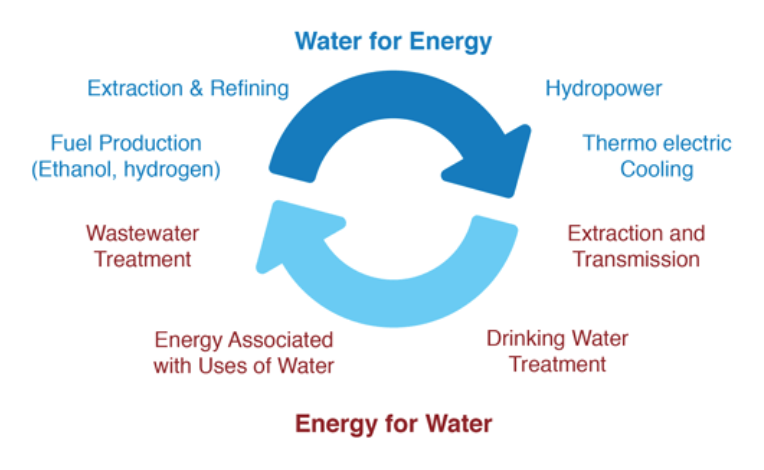
\includegraphics[width=4.5in]{figures/energy-water-nexus-perspectives.png}
       \caption[Perspectives on the Energy-Water Nexus]{Perspectives on the Energy-Water Nexus}
       \label{fig:energy-water-perspectives}
     \end{figure}
     
    The energy-water nexus is a term which has emerged from within the academic research community to describe these types of dynamic interrelationships which are inherent to our energy and water systems. There are two perspectives from which the energy-water nexus can be alternatively studied. The first emphasizes the \textit{water for energy} dimension, and is generally concerned with the study of processes and technologies that are involved with the direct withdrawal and consumption of water for the production of both primary and final energy resources. The second of these perspectives, and the one which shall be adopted for the purposes of this proposal, focuses instead on the \textit{energy for water} dimension; investigating processes and technologies which consume energy for the purpose of transmitting or purifying freshwater resources. 
    
     \begin{figure}[Dimensions of the Energy-Water Nexus]
       \centering
       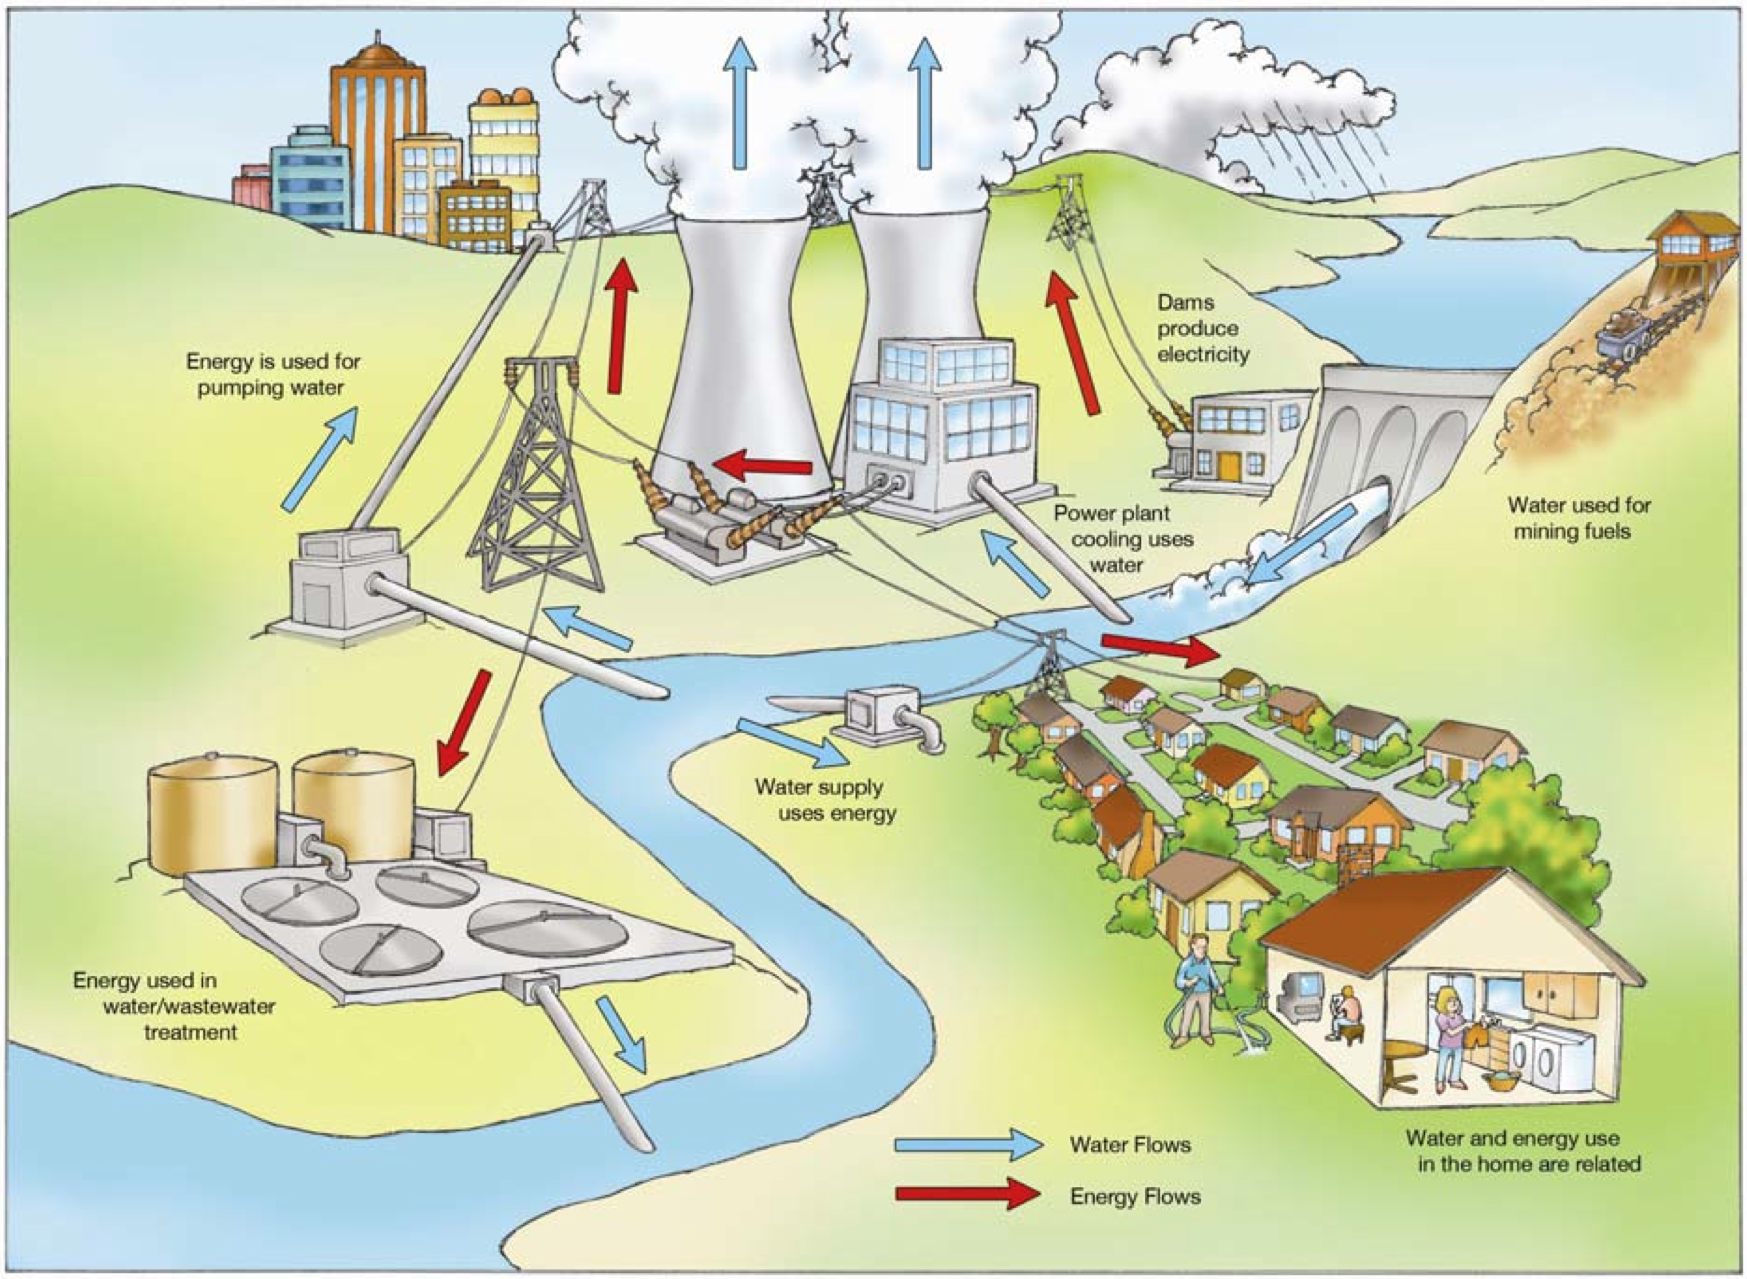
\includegraphics[width=5.5in]{figures/energy-water-nexus-dimensions.png}
       \caption[Dimensions of the Energy-Water Nexus]{The dimensions of the energy-water nexus}
       \label{fig:energy-water-dimensions}
     \end{figure}
    
Here in the United States, 50\% of total annual freshwater withdrawals are used for the cooling of thermoelectric power plants. Alternatively, 4\% of the nation's total energy consumption is dedicated to the transmission and purification of water and wastewater. While these national figures speak to the overall significance of this issue, the situation becomes more acute when one begins to consider different regional contexts. 
    
The criticality of the energy-water nexus becomes greatly exacerbated in those areas where either water is scarce, energy is scarce, or both. Unfortunately, the state of California suffers from both of these conditions to varying degrees, making the energy-water nexus a frequent source of regional interest within both the academic research and socio-political circles. For example, in a 2005 report published by the California Energy Commission (CEC) it was found that 19\% of the electricity and 32\% of the natural gas consumed within the entire state were used for purpose directly related to the supply and treatment of freshwater resources.
    
\section{Water Distribution Systems}
    
One of the main drivers for of this tremendous energy consumption within the state of California is the large scale transfer of freshwater resources between physically distinct hydrologic basins. California is crossed latitudinally by a massive network of interconnected hydraulic engineering projects including pipelines, aqueducts, reservoirs, and pump stations. These systems, which have been funded by a mixture of Federal, State, and Local agencies, were designed to reconcile discontinuities between the spatial and temporal distributions of the supply and demand for freshwater resources within the state.
    
Inter-basin transfers typically involve the movement of water against a considerable elevation gradient. Due to water's previously mentioned high density, there are substantial energetic costs associated with operating the infrastructure required to facilitate these transfers. For example, the bar graph to the right of Figure \ref{fig:infrastructure-energy-intensity} compares the energy intensity of several different sources of municipal water within the state of California. According to this research water resources which are supplied via inter-basin transfer, either through branches of the State Water Project or through the Colorado River Aqueduct, rank very poorly in terms of energy usage efficiency relative to a number of other water supply systems.
    
       \begin{figure}[The geographic extent of water distribution infrastructure in the state California]
       \centering
       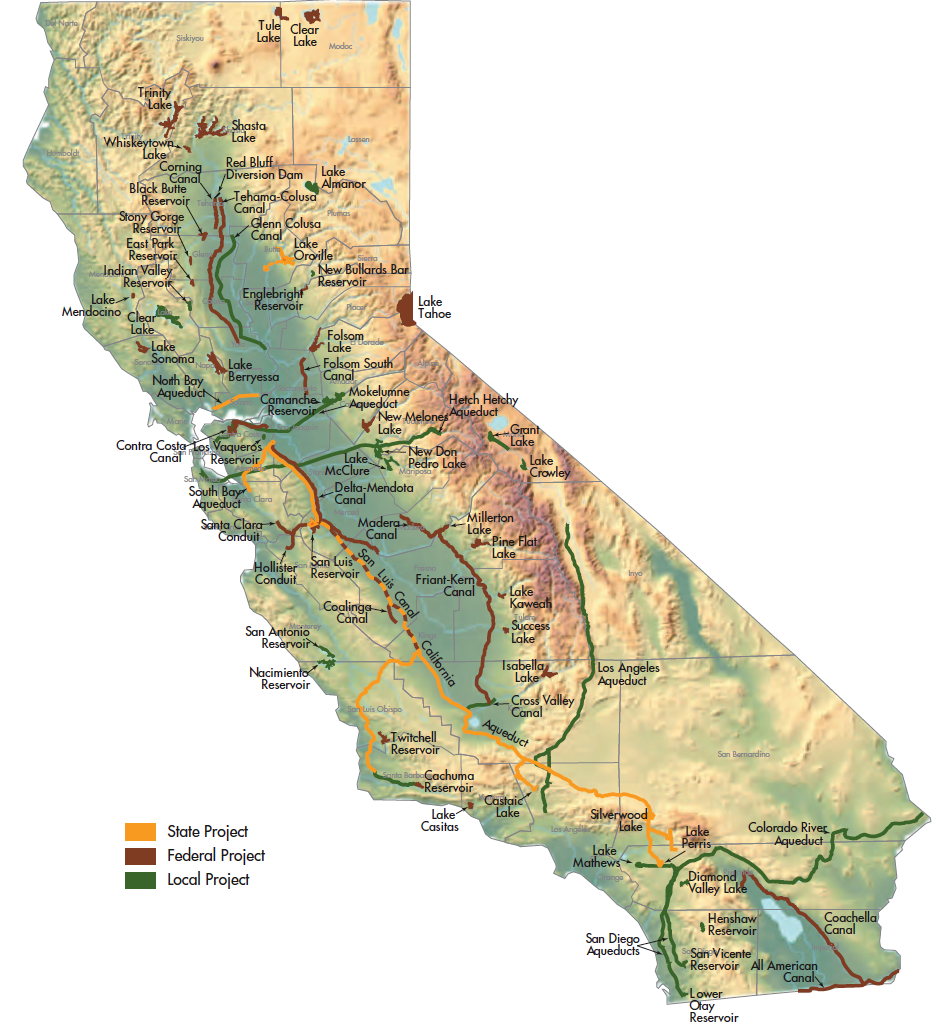
\includegraphics[width=5.5in]{figures/infrastructure.png}
       \caption[Characteristics of Water Distribution Infrastructure]{The geographic extent of water distribution infrastructure in the state of California}
       \label{fig:infrastructure-energy-intensity}
     \end{figure}
    
     \begin{figure}[The energy intensity of water distribution infrastructure in the state California]
       \centering
       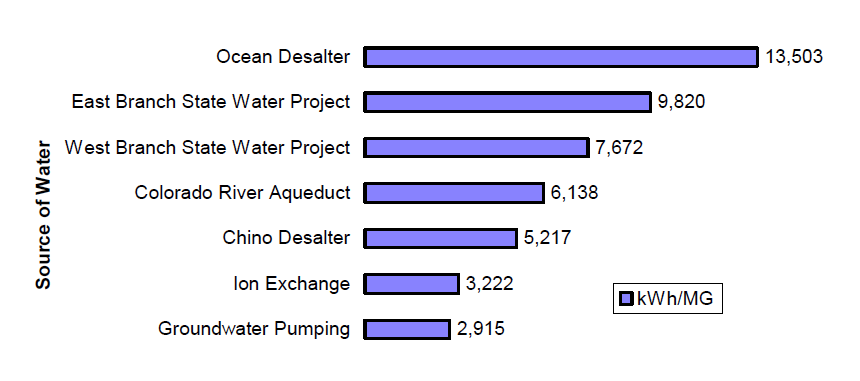
\includegraphics[width=5.5in]{figures/energy-intensity.png}
       \caption[Energy Intensity of Water Distribution Infrastructure]{The geographic extent of water distribution infrastructure in the state California}
       \label{fig:infrastructure-energy-intensity}
     \end{figure}
     
\section{Wastewater Treatment}

The term \textit{wastewater treatment} refers to a process of removing physical, chemical, or biological contaminants from a quantity of water such that their concentrations are sufficiently low for that quantity of water to be deemed fit for use in some specified application. Crucially implicit in this definition therefore, is the notion that the treatment methods, and any associated support systems involved, will vary on the basis of the purity requirements associated with the anticipated water end-use type. Figure provides a process flow diagram which demonstrates, in generic terms, the various phases of wastewater treatment and some of the methods/systems that are commonly used at each phase. Adjacent to this, on the right, is a list of common water end use types organized on the basis of the minimum degree of required pretreatment.

       \begin{figure}[Water consumed per unit power production for various electricity generation technologies]
       \centering
       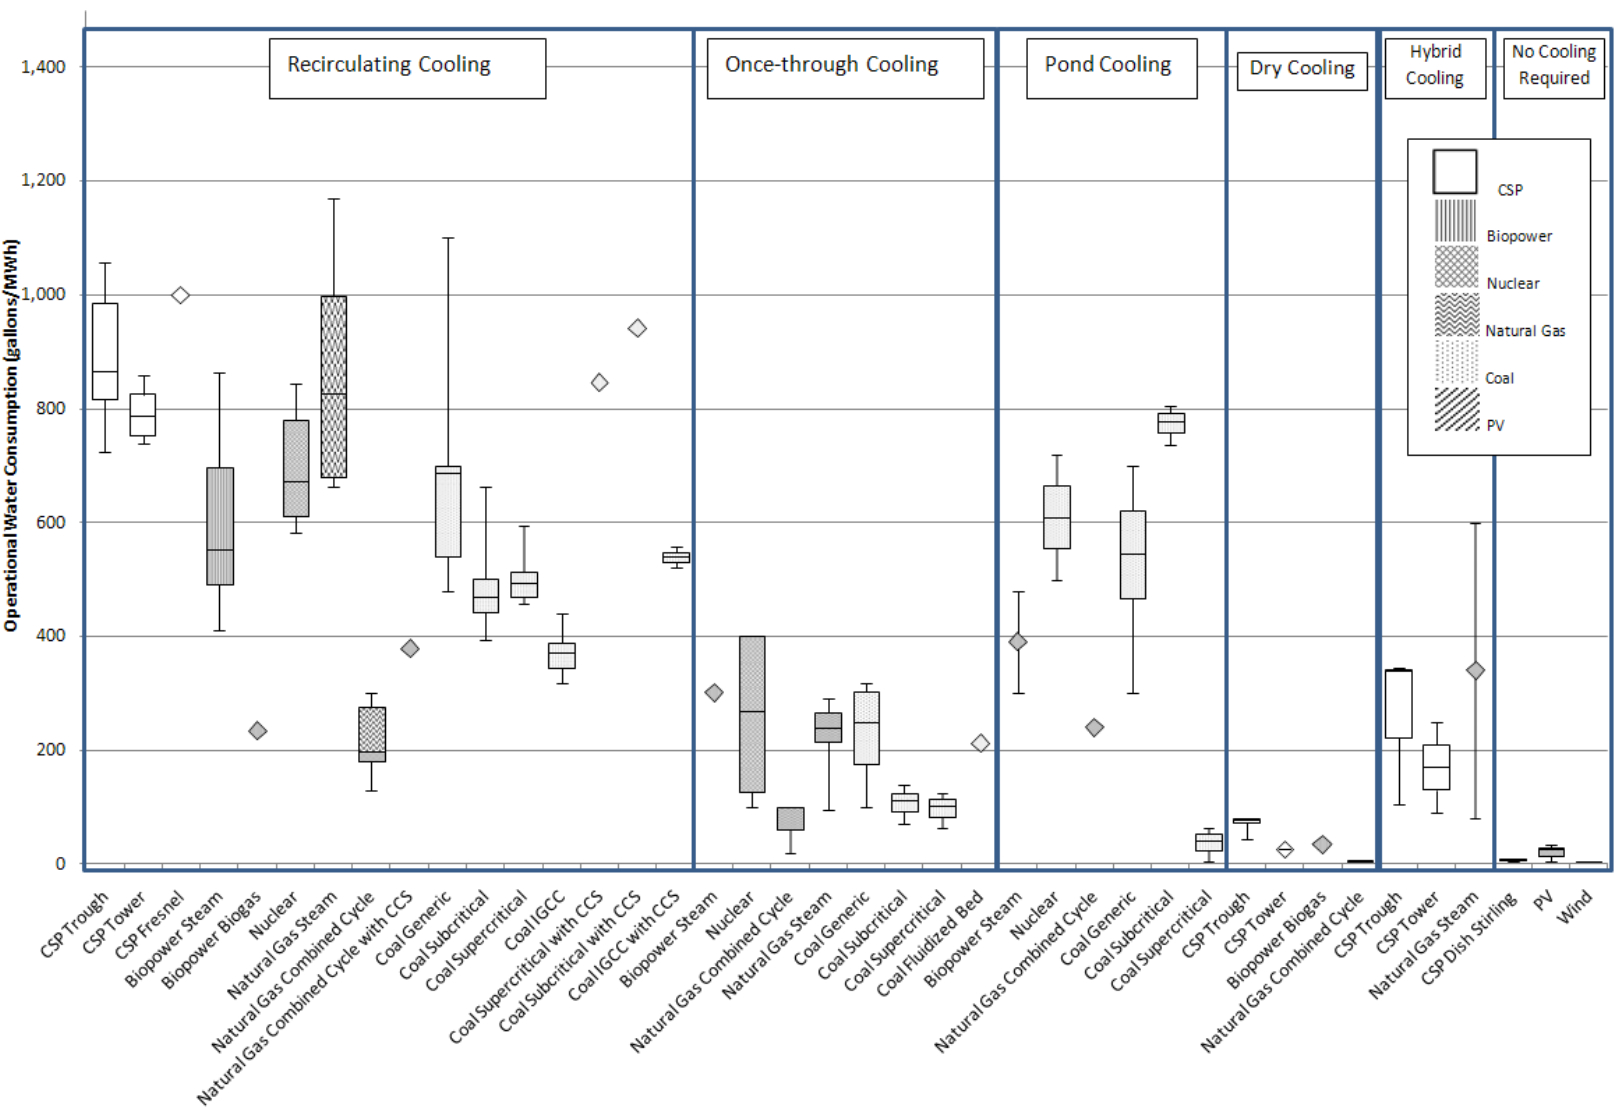
\includegraphics[width=5.5in]{figures/water_consumption_for_energy.png}
       \caption[Water Intensity of Energy Production]{The water consumption intensity, measured in terms of water consumed per unit power produced, for various electricity generation technologies}
       \label{fig:water-consumption-intensity}
        \end{figure}
    
\section{Wastewater Recycling and Reuse}
    
The fastest growing source of new water supply for municipal water districts in the Western United States is treated municipal wastewater. A major driver behind this trend has been the fact that treated municipal wastewater is perceived to be an energy efficient water supply option for a number of low quality uses, particularly when the end-use location is situated in close proximity to the wastewater treatment plant (WWTP). An illustrative example of such a condition might be the use of wastewater which had been subjected to basic secondary treatment for the irrigation of a nearby cemetery or golf course.
    
     \begin{figure}[Process flow diagram of various wastewater treatment methods]
       \centering
       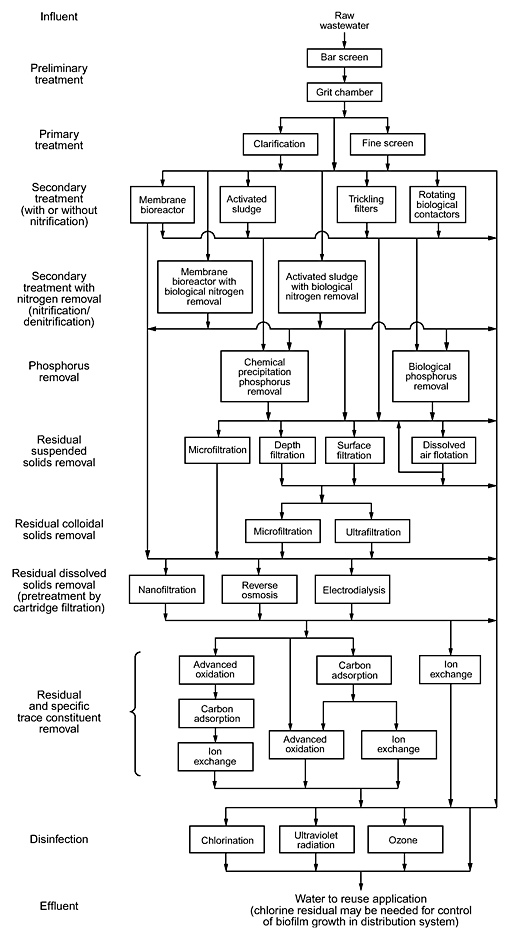
\includegraphics[width=3in]{figures/process-flow.png}
       \caption[Process Flow Diagram of Wastewater Treatment Methods]{Process flow diagram of various wastewater treatment methods}
       \label{fig:process-flow-diagram}
     \end{figure}
    
     \begin{figure}[End Use Categories for Recycled Water]
       \centering
       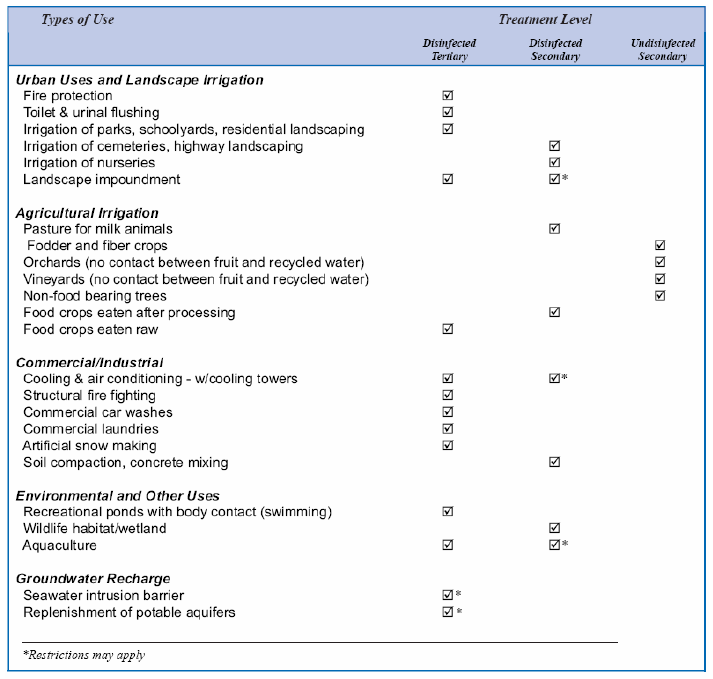
\includegraphics[width=5.5in]{figures/use-categories.png}
       \caption[End Use Categories for Recycled Water]{End Use Categories for Recycled Water}
       \label{fig:use-categories}
     \end{figure}        
              
 \section{Quantifying Life Cycle Energy-Water Usage Efficiency}

